% -----------------------------------------------
% Template for ISMIR Papers
% 2017 version, based on previous ISMIR templates

% Requirements :
% * 6+n page length maximum
% * 4MB maximum file size
% * Copyright note must appear in the bottom left corner of first page
% * Clearer statement about citing own work in anonymized submission
% (see conference website for additional details)
% -----------------------------------------------

\documentclass{article}
\usepackage{ismir,amsmath,cite,url}
\usepackage{graphicx}
\usepackage{color}
\usepackage{cleveref}
\usepackage{graphicx}
\usepackage{color}
\graphicspath{{figs/}}
\usepackage{booktabs}
\usepackage[inline]{enumitem}

\def\eg{\emph{e.g.\/}}
\def\ie{\emph{i.e.\/}}
\def\etc{\emph{etc.\/}}
\def\etal{\emph{et al.\/}}


% Title.
% ------
\title{Structured training for large-vocabulary chord recognition}

% Note: Please do NOT use \thanks or a \footnote in any of the author markup

% Single address
% To use with only one author or several with the same address
% ---------------
%\oneauthor
% {Names should be omitted for double-blind reviewing}
% {Affiliations should be omitted for double-blind reviewing}

% Two addresses
% --------------
%\twoauthors
%  {First author} {School \\ Department}
%  {Second author} {Company \\ Address}

%% To make customize author list in Creative Common license, uncomment and customize the next line
%  \def\authorname{First Author, Second Author}


% Three addresses
% --------------
\threeauthors
  {First Author} {Affiliation1 \\ {\tt author1@ismir.edu}}
  {Second Author} {\bf Retain these fake authors in\\\bf submission to preserve the formatting}
  {Third Author} {Affiliation3 \\ {\tt author3@ismir.edu}}

%% To make customize author list in Creative Common license, uncomment and customize the next line
%  \def\authorname{First Author, Second Author, Third Author}

% Four or more addresses
% OR alternative format for large number of co-authors
% ------------
%\multauthor
%{First author$^1$ \hspace{1cm} Second author$^1$ \hspace{1cm} Third author$^2$} { \bfseries{Fourth author$^3$ \hspace{1cm} Fifth author$^2$ \hspace{1cm} Sixth author$^1$}\\
%  $^1$ Department of Computer Science, University , Country\\
%$^2$ International Laboratories, City, Country\\
%$^3$  Company, Address\\
%{\tt\small CorrespondenceAuthor@ismir.edu, PossibleOtherAuthor@ismir.edu}
%}
%\def\authorname{First author, Second author, Third author, Fourth author, Fifth author, Sixth author}


\sloppy % please retain sloppy command for improved formatting

\begin{document}

%
\maketitle
%
\begin{abstract}
The abstract should be placed at the top left column and should contain about 150-200 words.
\end{abstract}
%
\section{Introduction}\label{sec:introduction}

% Chord recognition is maturing as a problem within MIR

% The gains to be had are now in the large-vocab regime (eg, tetrads/sevenths)

% These classes are rare in the common datasets, so modeling them is hard

% But we can leverage the structure of chord space to better exploit available data

\subsection{Our contributions}

In this work, we apply convolutional-recurrent neural networks to the problem of large-vocabulary chord recognition.
To exploit similarity between target chord classes, we introduce a structured representation of chord roots and quality into the model, which informs the chord tag prediction components.
Evaluation on a large collection of annotated music demonstrates that the proposed methods significantly improve upon prior work in modeling rare classes, while not sacrificing accuracy for common classes.

%
\section{Related work}

% 2016 - idealized chroma prediction, 25-class
\cite{korzeniowski2016feature} % idealized chroma -> logistic regression on small vocab

% 2015 - sigtia, RNN, 25-class
\cite{sigtia2015audio}

% 2014 - TMC (157)
\cite{cho2014improved} % k-stream HMM is a similar deal

% 2015 - four timely lessons (157)
\cite{humphrey2015four}


% 2012 - HPA (bass tracking), 25-class, 121-class
\cite{ni2012end} % HPA did bass tracking

% 2010 - chordino, 159 but not quite the same
\cite{mauchsimple}

\section{Methods}

% Use convolutional filters for local representation

% Use a bidrectional recurrent model to capture dynamics

% Predict chord label from latent state representation

%% either directly

%% or by first estimating (root, pitch classes, bass)

This section outlines the data preparation, architectures, and training strategies for the models under comparison.
We consider three independent design choices: one or two recurrent layers, the presence or absence of data augmentation, and the presence or absence of structured output training.
This results in eight model configurations, which are evaluated in the subsequent section.

\subsection{Encoder-decoder models}


The first chord recognition model uses a convolutional encoder, recurrent decoder architecture, as depicted in Figure~\ref{fig:model}. % FIXME citation needed
\begin{figure}
    \centering
    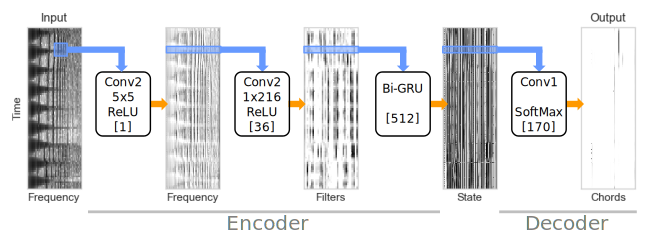
\includegraphics[width=0.95\columnwidth]{crnn1}
    \caption{Illustration of model architectures goes here.\label{fig:model}}
\end{figure}
Input audio is represented as a $T\times F$ time-series of log-power constant-Q spectra (for $T$ frames and $F$ frequency bands).
After batch normalization~\cite{ioffe2015batch}, the first convolutional layer consists of a single $5\times5$ filter, followed by a bank of $1\times F$ (full frequency range) convolutional filters, resulting in a $T\times 36$ feature encoding.
Both layers use rectified linear activations.
The first layer can be interpreted as a local harmonic saliency enhancer, as it tends to produce a filter which suppresses transients and vibrato while retaining sustained tones.
In preliminary experiments, we found that a single filter in the first layer was sufficient.
The second layer can be interpreted as a set of pitch class detectors, and we set the number of filters to allow 3 for each distinct pitch class.
The output of the second layer constitutes a convolutional encoding of the pitch class content for each input frame.

% TODO: refer to figure illustrating model parameters and/or activations


The convolutional feature encoding is mapped into either one or two layers of bi-directional gated recurrent units (GRUs)~\cite{cho2014learning}.
The GRU model is functionally similar to the commonly used long-short-term memory (LSTM) model~\cite{hochreiter1997long}, but has fewer parameters and often performs comparably in practice~\cite{jozefowicz2015empirical}.
The bi-directional variant consists of two independent recurrent models, one running in each direction, whose hidden state vectors are concatenated to produce the bi-directional hidden state vector $h(t)$ at frame $t$.
This layer integrates over the entirety of the input signal, and provides temporal smoothing and context for the encoded feature representation.
In the one-layer configuration (denoted as \emph{CRNN1}), the hidden state vector has total dimension 512 (256 for each direction).
In the two-layer configuration (denoted as \emph{CRNN2}), both layers have total hidden state dimensions 256, and the hidden state of the first layer serves as input to the second layer.


Finally, the hidden state vector $h(t)$ is decoded to the class label by a sigmoid layer, which produces a likelihood score $\hat{y}(t) \in [0, 1]^{V}$ over the chord vocabulary of $V$ symbols.
At each frame, the maximum likelihood label is selected, and the time-series of chord labels is run-length encoded to form the estimated annotation for the track.


% Figure for the basic model

% conv encoder, recurrent decoder model

% batch-norm on the cqt for standardization

% first filter = transient suppressor / local salience

% 3*12 full-height convolutional filters

% bidirectional recurrent model (GRU), d=128 in each direction

% logistic to output vocabulary


\subsection{Chord vocabulary}

\label{sec:vocab}
% For training the tag decoder, we map to a fixed vocabulary
%   1. discard missing / extra notes
%   2. discard inversions
%   3. split into (root, pitch classes)
%   4. match against quality templates:
%       - N
%       - maj, min, dim, aug
%       - min6, maj6
%       - min7, maj7, dom7, dim7, hdim7, minmaj7
%       - sus2, sus4
%       - X (unmatched)
%   5. resulting vocab = 12 * 14 + 2 = 170 classes
%

To train the decoder module, we map all labels in the training set to a finite vocabulary by the following procedure.
First, suppressed or extra notes are discarded, \eg:
\begin{align*}
    \texttt{D}\flat\texttt{:maj(*5,9)/3} &\mapsto \texttt{D}\flat\texttt{:maj/3}.
\end{align*}
Inversions are then discarded, \eg:
\begin{align*}
    \texttt{D}\flat\texttt{:maj/3} &\mapsto \texttt{D}\flat\texttt{:maj}.
\end{align*}
Next, labels are decomposed into \emph{root} and \emph{pitch classes} (relative to the root) using the encoding functionality provided by \texttt{mir\_eval}~\cite{raffel2014mir_eval}, \eg:
\begin{align*}
    \texttt{D}\flat\texttt{:maj} &\mapsto \begin{cases}
        1 & \text{root}\\
        (0, 4, 7) & \text{pitch classes}
    \end{cases}.
\end{align*}
The set of active pitch classes is matched against a set of 13 templates: \texttt{maj, min, dim, aug, min6, maj6, min7, maj7, dom7, hdim7, minmaj7, sus2, sus4}.
The root and matched template are combined, and mapped to a canonical form to resolve enharmonic equivalences:
\begin{align*}
    \left(1, (0, 4, 7) \right) &\mapsto \texttt{C}\sharp\texttt{:maj}.
\end{align*}
If the pitch class set does not match one of the templates, it is mapped to the unknown chord symbol \texttt{X}; the no-chord symbol is represented distinctly as \texttt{N}.
The final vocabulary contains 170 classes: 2 special symbols (\texttt{N, X}), and $12\times13=168$ combinations of root and quality.


\subsection{Structured training}

% Figure for the structured model

% Note: for structured training, no simplification is performed
%       so that the model can still learn to map power chords to major, for example
%       but the decoder component is still trained to map to the constrained vocab
%       even for chords that are out of vocab, we can still learn from their encoded representation 
%       and map them onto to a plausible output
%       

The direct model described above maps a hidden state vector $h(t)$ directly to a fixed vocabulary produced by the chord simplification strategy described in \cref{sec:vocab}, and is optimized by a na\"{\i}ve multi-class classification loss.
This approach has two clear drawbacks.
First, it does not account for the structure of chord space: for example, if the model predicts \texttt{B:maj} instead of \texttt{B:7}, it is penalized just as much as if it had predicted \texttt{C:maj} or \texttt{N}, even though it is far less severe of a mistake.
Second, the chord simplification strategy is \emph{lossy} in that it discards information such as suppressed or additional notes.
These effects combine to make modeling difficult, especially for rare classes.

To counteract these effects, we introduce a structured representation to the decoder component of the model.
We observe that the standard evaluation criteria for chord recognition operate over a decomposed representation of (\emph{root}, \emph{pitch classes}, \emph{bass}), as described in \cref{sec:vocab}~\cite{raffel2014mir_eval}.
This representation can be predicted directly by the model, and used either as direct output, or as an intermediate representation prior to decoding into the fixed vocabulary.

The structured models (denoted as \emph{CRNN1/2+S}) predict for each frame $t$ the root note (\texttt{A}--\texttt{G}$\sharp$, plus \texttt{N} for no-root), the bass note, and the active pitch classes from the hidden state vector $h(t)$.
Root and bass estimation use a soft-max non-linearity because the outputs are mutually exclusive (multi-class), while pitch class prediction uses a logistic non-linearity.
These three layers are concatenated, along with the hidden state itself, to produce the structured representation $s(t)$, from which the chord label is predicted.

During training, the structured models are provided with both the simplified chord tag, and the structured representation of the original (non-simplified) chord, and minimize the sum of losses across all outputs.
In this way, the model can both leverage the structure of the output space, and learn to be robust to errors or ambiguities in the vocabulary simplification process.


\subsection{Data augmentation}

% MUDA
%   training set is augmented with pitch shifts of +- n semitones for n in {1,2,\dots, 6}
%   muda does annotation deformation as well
% all augmentations of a track get the same importance weight
To increase training set variability, we apply pitch-shifting data augmentation using MUDA~\cite{mcfee2015software}.
For each training example, 12 deformations are generated by shifting up or down by between 1--6 semitones.
Testing and validation examples are not augmented.
Because since each observation exists in all twelve root classes, this provides a brute-force, approximate root invariance to the model.


\section{Evaluation}

% cite: ejh2015
%   1217, using the same 5-fold CV splits for comparison purposes
%   each training fold is split 75/25 for validation
%   training set => 12x by data augmentation
For evaluation, we used the dataset described by Humphrey and Bello~\cite{humphrey2015four}, which includes 1217 tracks from the Isophonics, Billboard, RWC Pop, and MARL collections.
To facilitate comparison with previous work, we retain the same 5-fold cross-validation splits, and randomly hold out 1/4 of each training set for validation.

\subsection{Pre-processing}

% features
%   librosa 0.5
Feature extraction was performed with librosa 0.5.0~\cite{librosa050}.
%   log cqt power, 36bpo, (C1 - C7) (260 bins)
Each track was represented as a log-power constant-Q spectrogram with 36 bins per octave, spanning 6 octaves starting at C1, and clipped at 80dB below the peak power for the entire track.
%   sr=44100, hop = 4096 => ~96ms frame rate
Signals were analyzed at 44.1KHz with a hop length of 4096 samples, resulting in a frame rate of approximately 10.8Hz.

\subsection{Training}
% training setup
All models are trained on 8-second patches (86 frames), though the models directly generalize to arbitrarily long inputs.
For tracks with multiple reference annotations, the output is selected uniformly at random from all references for each patch.
%   8sec patches (83 frames)
%   32 patches per batch
%   512 batches per epoch
Models are trained using mini-batches of 32 patches per batch, and 512 batches per epoch.
%   ADAM optimization
We use the ADAM optimizer~\cite{kingma2014adam}, and reduce the learning rate if there is no improvement in validation score after 10 epochs.
Training is stopped early if there is no improvement in validation score after 20 epochs, and limited to a maximum of 100 epochs total.
For all models, validation score is determined only by decoder loss (cross-entropy).

%   validation by decoder loss
%   learning rate reduction after 10 epochs
%   early stopping after 20 epochs
%   maximum 100 epochs

%   Keras + tensorflow
All models were implemented with Keras~2.0 and Tensorflow~1.0~\cite{chollet2015keras, tensorflow2015-whitepaper}.\footnote{Source code and pre-trained model parameters for our experiments will be made available upon publication.}

\subsection{Results}

\begin{figure*}[t]
    \centering
    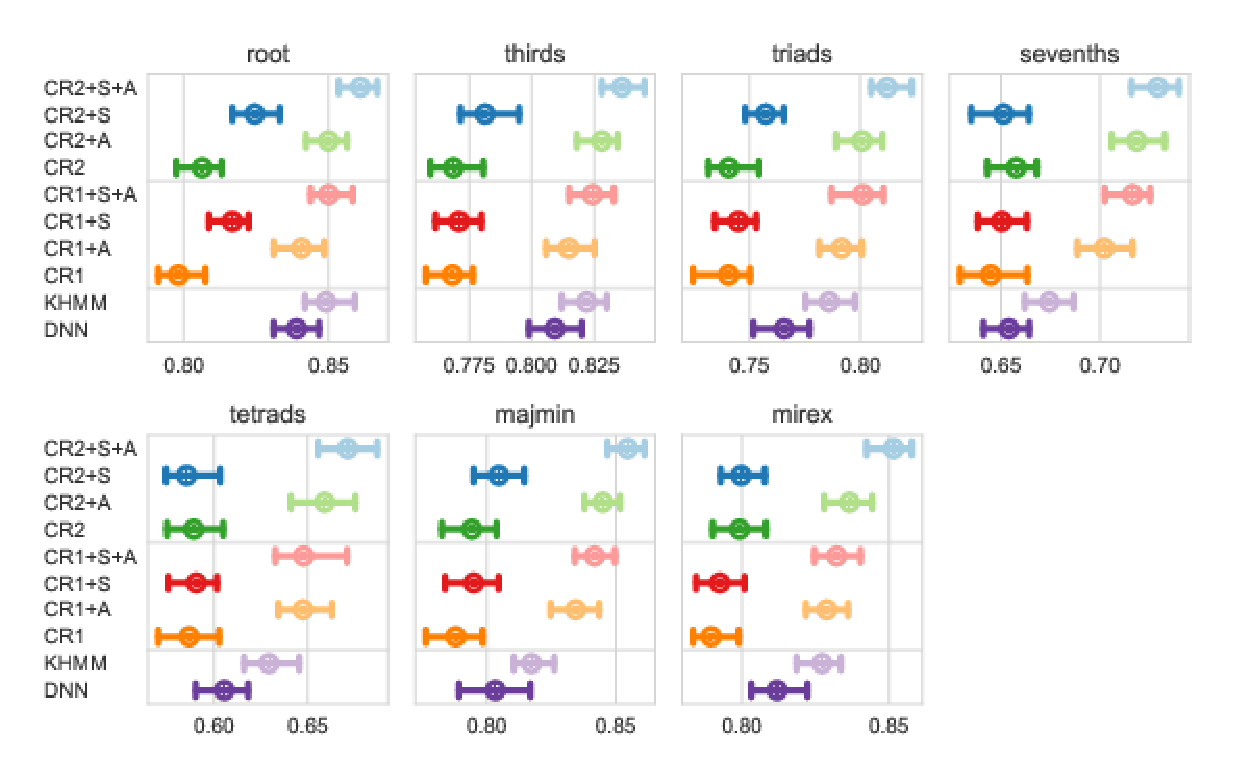
\includegraphics[width=0.9\textwidth]{crnn-scores}
    \caption{Weighted recall scores for all methods under comparison.  Each point represents the median score across all test points, with error bars covering the 95\% confidence interval estimated by bootstrap sampling.
        \emph{KHMM} denotes the K-stream HMM of Cho~\cite{cho2014improved}; \emph{DNN} denotes a convolutional network of Humphrey and Bello~\cite{humphrey2015four}.\label{fig:results}}
\end{figure*}
\section{Discussion}

% TODO:
%   feature visualization, analysis
%   error analysis
%   future work

%\section*{Acknowledgments}

% For bibtex users:
\bibliography{refs}

\end{document}
